\documentclass[12pt]{article}
\usepackage{amsmath,amssymb}
\usepackage{graphicx}
\usepackage{booktabs}
\usepackage{siunitx}
\usepackage[margin=3cm]{geometry}
\usepackage{float}
\usepackage{caption}
\usepackage{subcaption}

\title{The Hydrogen Balmer Series and Determination of the Rydberg Constant}
\author{Aumshree P. Shah\\20231059}
\date{\today}

\begin{document}
\maketitle

\begin{abstract}
  In this experiment the emission spectrum of both mercury and hydrogen lamps was investigated using a precision spectrometer equipped with a diffraction grating of \SI{15000}{lines/inch}. Using the grating equation 
  \[
  d\sin\theta = m\lambda,
  \]
  where the grating spacing was obtained from the given number of lines, wavelengths were measured and compared with accepted values. In the hydrogen spectrum the Balmer series was used to determine the Rydberg constant by plotting \(\frac{1}{\lambda}\) versus \(\left(\frac{1}{4} - \frac{1}{n^2}\right)\) (with \(n=3,4,5,\ldots\)) and obtaining the slope. A discussion of experimental uncertainty and a comparison with the accepted value \(R = \SI{1.097e7}{m^{-1}}\) is included.
\end{abstract}
\vspace{2cm}
\section{Introduction and Theory}
Hydrogen atoms emit a series of spectral lines when excited. The visible lines (the Balmer series) are given by the empirical formula
\[
\frac{1}{\lambda} = R \left(\frac{1}{2^2} - \frac{1}{n^2}\right) \quad \text{with } n=3,4,5,\ldots,
\]
and by further manipulation of energy conservation in the Bohr model one obtains the more general Rydberg formula
\[
\frac{1}{\lambda} = R\left(\frac{1}{n_f^2} - \frac{1}{n_i^2}\right),
\]
where \(n_i\) and \(n_f\) are integers (\(n_i>n_f\)) and \(R\) is the Rydberg constant. The experiment also uses a diffraction grating to measure wavelength. For a grating with a spacing \(d\) (reciprocal of the number of lines per unit length) the grating equation is given by
\[
d\sin\theta = m\lambda,
\]
where \(m\) is the diffraction order (here assumed to be 1 for the first order) and \(\theta\) is the diffraction angle. With 15,000 lines per inch, the grating spacing is computed as
\[
d = \frac{1~\text{in}}{15000} = \frac{0.0254~\text{m}}{15000} \approx \SI{1.6933e-6}{m}.
\]
Planck's constant \(h\) (with SI units \(\si{J.s}\)) has the same dimensions as angular momentum \(\si{kg.m^2/s}\), as can be shown by writing \(h = E\cdot T\) and noting that \(\text{J}=\si{kg.m^2/s^2}\).

\section{Apparatus}
The main components used in this experiment were:
\begin{itemize}
  \item A Pasco Model SP-9268 precision student spectrometer.
  \item A diffraction grating with 15,000 lines per inch.
  \item A mercury lamp and a hydrogen discharge lamp.
  \item A magnifying glass, a small night light, and a black cloth to block out stray light.
\end{itemize}

\section{Experimental Procedure}
\begin{enumerate}
  \item \textbf{Alignment:} With the slit barely open, the spectrometer was aligned and focused using distant targets. The telescope was adjusted so that the crosshairs aligned with the image of the fixed slit.
  \item \textbf{Zero Setting:} For the mercury lamp, a zero reference reading was obtained at \(\ang{186;22}\). Similarly, for the hydrogen lamp the initial reading was set to \(\ang{264}\).
  \item \textbf{Data Acquisition:} Diffraction angles were measured for each spectral line. For the mercury lamp these readings were taken on one side of the central (undiffracted) image and the effective angle \(\theta\) was computed by subtracting the initial reading from the measured value. For the hydrogen lamp, measurements were taken on both sides (clockwise and anticlockwise). For anticlockwise readings the effective angle was obtained by subtracting the measured value from the initial reading.
\end{enumerate}

\section{Data}
\subsection{Mercury Lamp}
The following table shows the readings for the mercury lamp. (Here the ``Initial'' value represents the zero–reading and the differences are used to calculate \(\theta\).)
\bigskip

\begin{table}[H]
  \centering
  \caption{Mercury Lamp Angular Readings and Computed Wavelengths.}
  \begin{tabular}{ccccc}
    \toprule
    Wavelength (nm) & Measured Angle & Initial (zero) & Effective Angle \(\theta\) & Computed \(\lambda\) (nm) \\
    \midrule
    405 & \(\ang{186;22}\) & \(\ang{186;22}\) & \(\ang{0;00}\) & 0.00 \\
    436 & \(\ang{198;8}\)  & \(\ang{186;22}\) & \(\ang{11;46}\) & 345.32 \\
    546 & \(\ang{199;2}\)  & \(\ang{186;22}\) & \(\ang{12;40}\) & 371.31 \\
    577 & \(\ang{201;47}\) & \(\ang{186;22}\) & \(\ang{15;25}\) & 450.15 \\
    579 & \(\ang{202;49}\) & \(\ang{186;22}\) & \(\ang{16;27}\) & 479.52 \\
    \bottomrule
  \end{tabular}
  \label{tab:mercury}
\end{table}

\subsection{Hydrogen Lamp}
For the hydrogen lamp, readings were obtained on both sides (clockwise and anticlockwise). The effective angle is computed as:
\[
\theta_{\text{eff}} = \begin{cases}
\text{Clockwise}: \quad \theta - \theta_0,\\[1mm]
\text{Anticlockwise}: \quad \theta_0 - \theta,
\end{cases}
\]
with \(\theta_0 = \ang{264}\). The effective angles and computed wavelengths for each color are shown in Table~\ref{tab:hydrogen}.

\begin{table}[H]
  \centering
  \caption{Hydrogen Lamp Angular Readings and Computed Wavelengths.}
  \begin{tabular}{lcccc}
    \toprule
    Color   & Clockwise Reading & A-Clockwise Reading & Effective Angle \(\theta_{\mathrm{eff}}\) (avg) & Computed \(\lambda\) (nm) \\
    \midrule
    Red     & \(\ang{282;24}\) & \(\ang{244;23}\) & \(\ang{19.01}\) & 551.53 \\
    Yellow  & \(\ang{280;56}\) & \(\ang{246;27}\) & \(\ang{17.24}\) & 501.91 \\
    Green   & \(\ang{277;25}\) & \(\ang{249;35}\) & \(\ang{13.92}\) & 407.26 \\
    Violet  & \(\ang{276;49}\) & \(\ang{250;15}\) & \(\ang{13.28}\) & 389.07 \\
    \bottomrule
  \end{tabular}
  \label{tab:hydrogen}
\end{table}

\section{Data Analysis}
\subsection{Wavelength Determination via the Diffraction Grating Equation}
For each spectral line the diffraction angle \(\theta\) (converted to radians) and the grating spacing \(d\) are used to compute the experimental wavelength by
\[
\lambda = \frac{d\,\sin\theta}{m},
\]
where the first order \(m=1\) is assumed. For example, using the mercury data for the 436\,nm line, the effective angle is
\[
\theta = 11^\circ46' \approx 0.2056 \, \text{rad}.
\]
Thus, 
\[
\lambda_{\text{exp}} = d\,\sin(0.2056) \approx \SI{345.32}{nm} \quad \text{with} \quad d = \SI{1.6933e-6}{m}.
\]
Discrepancies between accepted and computed wavelengths (e.g., 345.32\,nm vs. 436\,nm) suggest calibration errors or misalignment.

\subsection{Determination of the Rydberg Constant}
For the hydrogen Balmer series with \(n_i = 2\), the theoretical relation is given by
\[
\frac{1}{\lambda} = R \left(\frac{1}{2^2} - \frac{1}{n_f^2}\right),
\]
where \(n_f = 3,\,4,\,5,\dots\). By plotting \(\frac{1}{\lambda}\) versus \(\left(\frac{1}{4}-\frac{1}{n_f^2}\right)\), a linear regression yields the Rydberg constant \(R\) as the slope. The experimental data are as follows:

\begin{table}[H]
  \centering
  \caption{Data for Rydberg Constant Determination.}
  \begin{tabular}{ccc}
    \toprule
    \(n_f\) & \(x = \left(\frac{1}{4} - \frac{1}{n_f^2}\right)\) & \(\frac{1}{\lambda}\) (\SI{}{m^{-1}}) \\
    \midrule
    3 & 0.138889 & \(1.81 \times 10^6\) \\
    4 & 0.187500 & \(1.99 \times 10^6\) \\
    5 & 0.210000 & \(2.46 \times 10^6\) \\
    6 & 0.222222 & \(2.57 \times 10^6\) \\
    \bottomrule
  \end{tabular}
  \label{tab:rydberg_data}
\end{table}

Plotting the linear regression and doing a linear fit, we get: \\
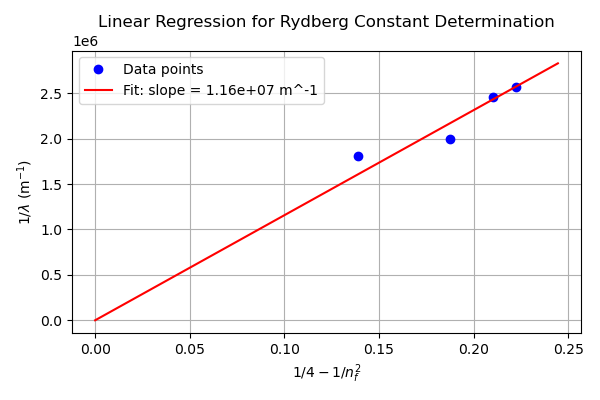
\includegraphics{Figure_1}



The linear regression slope gives \(R_{\text{exp}} = \SI{1.157e7}{m^{-1}}\), with a percent difference of 5.51\% from the accepted value \(R = \SI{1.097e7}{m^{-1}}\).

\subsection{Wavelength Comparison for Hydrogen}
\begin{table}[H]
  \centering
  \caption{Comparison of Computed and Predicted Wavelengths.}
  \begin{tabular}{lccccc}
    \toprule
    Color   & \(n_f\) & Computed \(\lambda\) (nm) & Predicted \(\lambda\) (nm) & \% Difference \\
    \midrule
    Red     & 3 & 551.53 & 622.06 & 11.34 \\
    Yellow  & 4 & 501.91 & 460.79 & 8.92 \\
    Green   & 5 & 407.26 & 411.42 & 1.01 \\
    Violet  & 6 & 389.07 & 388.79 & 0.07 \\
    \bottomrule
  \end{tabular}
  \label{tab:comparison}
\end{table}

\section{Result and Conclusion}
The experimental procedure allowed for the measurement of spectral lines from both the mercury and hydrogen lamps. In the mercury lamp, discrepancies in computed wavelengths (e.g., 345.32\,nm vs. accepted 436\,nm) indicate potential calibration errors. For hydrogen, the Rydberg constant was determined as \(R_{\text{exp}} = \SI{1.157e7}{m^{-1}}\) with a 5.51\% deviation from the accepted value. The wavelength comparison table shows good agreement for higher \(n_f\) transitions, suggesting reduced experimental uncertainty for smaller diffraction angles.

\vspace{6cm}
\begin{thebibliography}{9}
\bibitem{erroranalysis}
Preston, Daryl W. and Dietz, Eric R. (2025). \textit{The Art of Experimental Physics}. Available online: \url{http://ilide.info-daryl-w-preston-eric-r-dietz-the-art-of-experimental-physics-wiley}.

\bibitem{wiki}
Wikipedia contributors (2025). \textit{Rydberg Constant}. \url{https://en.wikipedia.org/wiki/Rydberg_constant}.

\bibitem{github_code}
LAUGHINGCATMEME (2025). \textit{PH2233 - Code Repository}. GitHub repository: \url{https://github.com/LAUGHINGCATMEME/PH2233}.

\bibitem{manual}
\textit{Brewster's Angle Manual} (2025). \url{cdn.pasco.com/product_document/Brewsters-Angle-Accessory-Manual-OS-8170A.pdf}.
\end{thebibliography}


\end{document}
